\chapter{Evaluierung}
\label{ch:evaluierung}

Verglichen mit mathematischen Berechnungen sind computerlinguistische Aufgabenstellungen weniger deterministisch und es ist weniger offensichtlich, was die \emph{richtige} Antwort ist.  Aus diesem Grunde sollen die Zwischen- und Endergebnisse des Programms mittels stichprobenartiger Betrachtungen und Untersuchungen hinsichtlich Auffälligkeiten ausgewertet werden. 

Für die Evaluierung der erzeugten RDF-Dateien wurden zudem von einem Teil der verarbeiteten Texte manuell RDF-Dateien zum Abgleich erzeugt. Für diese RDF-Dateipaare wurde Precision und Recall ermittelt.


\section{FZ 1.4 Evaluierung zur Vorverarbeitung medizinischer Texte}
\label{sec:FZ1.4} 

Zur Evaluierung des Preprocessors wurden sowohl allgemeine Untersuchungen des Preprocessors angestellt als auch eine Analyse des Sentence Boundary Detectors \emph{PySBD} durchgeführt.

\subsection{Allgemeine Evaluation des Preprocessors}
\label{sec:evaluation_preprocessor}

Ziel des Preprocessors ist es, die gegebenen Texte so umzuwandeln, dass der anschließend angewandte SpaCy-Sentencizer den Text in möglichst sinnvolle Sätze aufteilt, die dann weiterverarbeitet werden. Ein Hauptaugenmerk während der Implementierung lag auf der sinnvollen Aufteilung von Aufzählungen. Wie schon im Kapitel \ref{ch:implementierung} geschrieben gelingt das.

Ohne den Preprocessor würde man der weiteren Verarbeitung z. B. den \glqq Satz\grqq aus dem \emph{TextToAnalyze.txt} übergeben:

\begin{quotation}
	\glqq Psychological symptoms\verb!\n!\verb!\n!The psychological symptoms of depression include:\verb!\n!- continuous low mood or sadness\verb!\n!- feeling hopeless and helpless\verb!\n!- having low self-esteem\verb!\n!- feeling tearful\verb!\n!- feeling guilt-ridden\verb!\n!- feeling irritable and intolerant of others\verb!\n!- having no motivation or interest in things\verb!\n!- finding it difficult to make decisions\verb!\n!- not getting any enjoyment out of life\verb!\n!- feeling anxious or worried\verb!\n!- having suicidal thoughts or thoughts of harming yourself\verb!\n!\verb!\n!Physical symptoms\verb!\n!\verb!\n!The physical symptoms of depression include:\verb!\n!- moving or speaking more slowly than usual\verb!\n!- changes in appetite or weight (usually decreased, but sometimes increased)\verb!\n!- constipation\verb!\n!- unexplained aches and pains\verb!\n!- lack of energy\verb!\n!- low sex drive (loss of libido)\verb!\n!- changes to your menstrual cycle\verb!\n!- disturbed sleep – for example, finding it difficult to fall asleep at night or waking up very early in the morning\verb!\n!\verb!\n!Social symptoms\verb!\n!\verb!\n!The social symptoms of depression include:\verb!\n!- avoiding contact with friends and taking part in fewer social activities\verb!\n!- neglecting your hobbies and interests\verb!\n!- having difficulties in your home, work or family life\verb!\n!\verb!\n!Severities of depression\verb!\n!\verb!\n!Depression can often come on gradually, so it can be difficult to notice something is wrong.\grqq
\end{quotation} 

Mit Anwendung des Preprocessors übergibt man stattdessen die folgenden Sätze:
\begin{enumerate}
	\item \glqq The psychological symptoms of depression include continuous low mood or sadness.\verb!\n!\grqq
	\item \glqq The psychological symptoms of depression include feeling hopeless and helpless.\verb!\n!\grqq
	\item \glqq The psychological symptoms of depression include having low self esteem.\verb!\n!\grqq
	\item \glqq The psychological symptoms of depression include feeling tearful.\verb!\n!\grqq
	\item \glqq The psychological symptoms of depression include feeling guilt ridden.\verb!\n!\grqq
	\item \glqq The psychological symptoms of depression include feeling irritable and intolerant of others.\verb!\n!\grqq
	\item \glqq The psychological symptoms of depression include having no motivation or interest in things.\verb!\n!\grqq
	\item \glqq The psychological symptoms of depression include finding it difficult to make decisions.\verb!\n!\grqq
	\item \glqq The psychological symptoms of depression include not getting any enjoyment out of life.\verb!\n!\grqq
	\item \glqq The psychological symptoms of depression include feeling anxious or worried.\verb!\n!\grqq
	\item \glqq The psychological symptoms of depression include having suicidal thoughts or thoughts of harming yourself.\verb!\n!\grqq
	\item \glqq Physical symptoms.\verb!\n!\grqq
	\item \glqq The physical symptoms of depression include moving or speaking more slowly than usual.\verb!\n!\grqq
	\item \glqq The physical symptoms of depression include changes in appetite or weight (usually decreased, but sometimes increased).\verb!\n!\grqq
	\item \glqq The physical symptoms of depression include constipation.\verb!\n!\grqq
	\item \glqq The physical symptoms of depression include unexplained aches and pains.\verb!\n!\grqq
	\item \glqq The physical symptoms of depression include lack of energy.\verb!\n!\grqq
	\item \glqq The physical symptoms of depression include low sex drive (loss of libido).\verb!\n!\grqq
	\item \glqq The physical symptoms of depression include changes to your menstrual cycle.\verb!\n!\grqq
	\item \glqq The physical symptoms of depression include disturbed sleep for example, finding it difficult to fall asleep at night or waking up very early in the morning.\verb!\n!\grqq
	\item \glqq Social symptoms.\verb!\n!\grqq
	\item \glqq The social symptoms of depression include avoiding contact with friends and taking part in fewer social activities.\verb!\n!\grqq
	\item \glqq The social symptoms of depression include neglecting your hobbies and interests.\verb!\n!\grqq
	\item \glqq The social symptoms of depression include having difficulties in your home, work or family life.\verb!\n!\grqq
	\item \glqq Severities of depression.\verb!\n!\grqq
	\item \glqq Depression can often come on gradually, so it can be difficult to notice something is wrong.\verb!\n!\grqq 
\end{enumerate}

Der Preprocessor wurde unter Berücksichtigung der gewählten Beispieltexte aufgebaut. Diese Texte haben alle eine ähnliche Struktur (z. B. viele Texte mit Aufzählungen, wenige Literaturangaben, keine Dialog-Texte). Es kann sein, dass Texte mit stark abweichender Struktur von dem Preprocessor nicht optimal verarbeitet werden.

Während der Evaluation des Preprocessors wurde getestet, wie sich die Ergebnisse des MedExtractors unterscheiden, wenn man die Texte mit dem Preprocessor vorverarbeitet bzw. dies nicht tut. 
Dabei ist aufgefallen, dass ohne die Vorverarbeitung des Preprocessors (d. h. wenn die Texte nur mit dem SpaCy-Sentencizer aufgeteilt werden), anschließend mehr Einträge in der resultierenden KnowledgeBase gespeichert sind. Dieser Test wurde auf zwei verschiedenen Textmengen durchgeführt. Die Anzahl der jeweiligen KnowledgeBase-Einträge sind in folgender Tabelle dokumentiert:

\begin{tabular}[h]{lrr}
	\hline
	 & mit Preprocessing & ohne Preprocessing\\
	 \hline
	Textmenge 1 & 1566 & 2089 \\
	Textmenge 2 & 432 & 903\\
	\hline
\end{tabular}\\

Bei einer Weiterentwicklung des Preprocessors sollte näher untersucht werden wodurch diese Unterschiede entstehen und überlegt werden, wie man damit umgeht.

\subsection{PySBD}
\label{evaluation_pysbd}
PySBD (\cite{sadvilkar_pysbd_2020}) ist ein regelbasierter \emph{Sentence Boundary Detector/Disambiguater} (Satzgrenzen-Finder). Die Entwicklung von PySBD basiert auf einem Golden Rule Set (\cite{golden_rules}). Diese Golden Rules sind Spezialfälle in Sätzen, nach deren richtiger Bearbeitung ein Sentence Boundary Detector beurteilt werden kann. Eine der Golden Rules ist zum Beispiel\\

\begin{quotation}
	\textbf{\glqq U.S. as non sentence boundary\grqq}\\
	I have lived in the U.S. for 20 years. \\
	=> [\glqq I have lived in the U.S. for 20 years.\grqq]
\end{quotation}

Im Vergleich mit anderen Sentence Boundary Detectors erfüllt PySBD diese Golden Rules sehr gut, siehe \cite{sadvilkar_pysbd_2020}.

\subsubsection{Vergleich der Einteilung von Texten in Sätze mit und ohne PySBD}
Es soll untersucht werden worin die Vor- und Nachteile beim Einteilen von Texten in Sätze mit der Bibliothek \emph{PySBD} liegen. 
Alternativ gibt es die Möglichkeit den Sentencizer von SpaCy zu nutzen. Für den Vergleich wird die Verarbeitung der 51 Texte in 
\emph{medextractor/resources/to\_analyze} verglichen. Dies geschieht in der python-Datei \emph{test/pysbd\_evaluation\_sentences.py}.\\

Es fällt schnell auf, dass der Hauptunterschied in der Einteilung von Texten in einzelne Sätze mit und ohne PySBD darin besteht, 
dass ein Zeilenumbruch unterschiedlich interpretiert wird.
Aus dem folgenden Textabschnitt in der Datei \emph{agorophobia.txt}\\

\begin{quotation}
	\glqq \verb!\n!Symptoms - Agoraphobia\verb!\n!\verb!\n!The severity of agoraphobia can vary significantly between individuals.\grqq
\end{quotation}

erhält man mit dem SpaCy Sentencizer zum Beispiel den Satz

\begin{quotation}
	\glqq \verb!\n!Symptoms - Agoraphobia\verb!\n!\verb!\n!The severity of agoraphobia can vary significantly between individuals.\grqq,
\end{quotation}

während die Aufteilung in Sätze mit PySBD folgendermaßen aussieht:

\begin{enumerate}
	\item \glqq Symptoms - Agoraphobia\verb!\n!\verb!\n!\grqq
	\item \glqq The severity of agoraphobia can vary significantly between individuals.\verb!\n!\verb!\n!\grqq
\end{enumerate}

Insgesamt wird von den 51 Texten nur einer vom PySBD- und SpaCy-Sentencizer auf die gleiche Art in Sätze eingeteilt.\\
Wendet man nun die folgende Art der Nachverarbeitung der Texte an:
\begin{enumerate}
	\item Sätze, die ein \glqq \verb!\n!\grqq enthalten, werden an dieser Stelle in zwei Sätze aufgesplittet,
	\item Leerzeichen am Anfang und am Ende von Sätzen werden entfernt,
	\item leere Sätze werden entfernt,
\end{enumerate}
 werden schon 41 der 51 Texte komplett gleich verarbeitet. Ausnahmen bilden dann (fast) nur noch Sätze, die Zeichen wie z.B. \glqq ]\grqq, \glqq :\grqq und \glqq -\grqq enthalten (diese speziellen Zeichen werden vom PySBD- und SpaCy-Sentencizer unterschiedlich behandelt), oder Satzanfänge ohne vorhergehendes Leerzeichen.\\

 
\subsubsection{Fazit zu PySBD}
Der Preprocessing-Schritt des MedExtractors enthält nicht nur das Erkennen von Satzgrenzen, sondern noch weitere Schritte um die Sätze so umzuformen, dass sie in der weiteren Verarbeitung mit dem MedExtractor gut genutzt werden können (siehe Kapitel [TODO]). Für die Zwecke des MedExtractors und für die zur Evaluierung genutzten Texte war PySBD sehr hilfreich. Während der Evaluierung ist aber auch aufgefallen, dass mit Berücksichtigung der Eigenheiten des SpaCy Sentencizers wahrscheinlich ähnlich gute Ergebnisse im Preprocessing-Schritt hätten erzielt werden können. Somit kann PySBD für die Zwecke des MedExtractors zwar empfohlen werden, mit anderen Sentence Boundary Detectorn könnten aber voraussichtlich ähnlich gute Ergebnisse erzielt werden. \\
In der weiteren Entwicklung des Preprocessors, bzw. des MedExtractors, könnte man versuchen mit einer besseren Einstellung der Parameter von PySBD bessere Ergebnisse zu erzielen, oder mit einem anderen \emph{Sentence Boundary Detector} (mehrere Alternativen werden in \cite{sadvilkar_pysbd_2020} genannt) zu arbeiten.





\section[FZ 2.5 Evaluierung zur Überführung med. Fachvokabulars]{FZ 2.5 Evaluierung zur Überführung medizinischen Fachvokabulars in maschinenlesbare Form zur weiteren Verarbeitung durch NLP}
\label{sec:FZ2.5}

Für die \emph{Named Entity Recognition} ist der \emph{EntityRuler} das einfachste Mittel, das von \emph{spaCy} angeboten wird. Der \emph{Entity Ruler} sucht konventionell die trainierten Begriffe im Text, wobei bei Mehrdeutigkeit / Überlappungen der jeweils längste Ausdruck (gemessen an der Anzahl der Worte) oder, wenn dies nicht eindeutig ist, der als erstes auftretende Ausdruck angezeigt wird. Der \emph{Entity Ruler} benötigt keine Trainingssätze und ist daher für das MedExtractor-Projekt am Anfang besser geeignet als der auf statistischen Modellen basierende \emph{Entity Recognizer}.

Mit den Exporten für den \emph{Entity Linker} steht nun aber eine größere Anzahl von Trainingsätzen zur Verfügung und es stellt sich die Frage, ob diese ein Training des \emph{Entity Recognizers} erlauben, so dass dieser zuverlässig Entitäten erkennt.

In dem Jupyter Notebook \emph{entity\_recognizer\_demo.ipynb} werden \emph{Entity Ruler} und \emph{Entity Recognizer} gegenübergestellt. Die Trainingsdaten stammen in beiden Fällen aus der Datei \emph{all\_entity\_linker\_export.xml}. Diese wiederum wurden vom MedExtractor aus den drei Quellen extrahiert, die auch in Abschnitt \ref{subsec:detaillierteAuswertung} analysiert werden (vgl. Tabelle \ref{tab:zaehlung}). Als Test-Text wurde der englischsprachige Artikel über \emph{Agoraphobie} auf Wikipedia verwendet, der nicht Teil der drei Quellen ist, aus denen die Trainingsdaten stammen.

Der \emph{Entity Ruler} findet 105 und der \emph{Entity Recognizer} 98 Entitäten. Überwiegend decken sich die Ergebnisse von \emph{Entity Ruler} und \emph{Entity Recognizer}. Jedoch findet der \emph{Entity Recognizer} 12 Entitäten, die nicht trainiert wurden und falsch sind. Dazu gehören z.B. die Begriffe \emph{scholar}, \emph{social sciences}, \emph{prone} oder \emph{tense}, die vom neuronalen Netz fälschlich als Entitäten identifiziert werden.

Interessanterweise findet der \emph{Entity Recognizer} den Begriff \emph{suicide ideation} (Suizidgedanken), obwohl dieser Begriff nicht im trainierten Vokabular enthalten ist. Das in dieser Arbeit aus der \emph{MetaMapLite}-Datenbank abgeleitete Trainingsvokabular kennt nur die Pluralform \emph{suicidal ideations} und verwendet das Wort \emph{suicidal} anstelle von \emph{suicide}. Daher findet der MedExtractor den Begriff nicht in dem Wikipedia-Text über Agoraphobie und auch nicht in den anderen Texten, die von ihm analysiert wurden, so dass er nicht in der Wissensrepräsentation und auch nicht in der Datei \emph{all\_entity\_linker\_export.xml} enthalten ist. Auch den Begriff \emph{suicide} findet der MedExtractor nicht, da dieses Wort nicht im Symptom-Vokabular enthalten ist.

In den vom MedExtractor gefundenen Trainingssätzen kommt der Begriff \emph{suicidal ideation} im Singular dagegen mehrfach vor, da der MedExtractor in diesen Sätzen andere Symptome gefunden hat. Man mag in dem Umstand, dass der \emph{Entity Recognizer} den Begriff \emph{suicide ideation} findet, ein `intelligentes' Verhalten des zugrundeliegenden neuronalen Netzes sehen. Jedoch zeigt der Vergleich insgesamt, dass der \emph{Entity Ruler} zuverlässiger arbeitet als der \emph{Entity Recognizer}. Um die Vorteile eines statistischen Modells nutzen zu können (z.B. kontextsensitive Worterkennung), bedarf es offenbar noch mehr Trainingsdaten.








\section{FZ 3.4 Evaluierung zur Wissensrepräsentation}
\label{sec:FZ3.4} 
In Abschnitt \ref{subsec:RDF-Vergleich} erfolgt eine statistische Auswertung der Vergleichsergebnisse von manuell und mit dem MedExtractor erstellten RDF-Dateien. Danach werden diese und weitere beim stichprobenartigen Sichten der MedExtractor-Ergebnisse gefundene Erkenntnisse in Abschnitt \ref{subsec:detaillierteAuswertung} diskutiert.




\subsection{Vergleich der manuell und vom MedExtractor erstellten RDF-Dateien}
\label{subsec:RDF-Vergleich} 

Zur Evaluierung des Systems wurden von zehn der verwendeten Texte manuelle RDF-Dateien erstellt, um diese mit dem vom MedExtractor erstellten RDF-Dateien zu vergleichen. 

Da der MedExtractor Krankheiten Symptome zuordnet, wurden ebenso bei der manuellen Dateierstellung aus den Texten Symptome ausgewählt, die in die RDF-Dateien aufgenommen wurden. Diese manuelle Erstellung erfordert jedoch Augenmaß, da es kein absolutes Kriterium dafür gibt, was als Symptom einer Krankheit anzusehen ist. Insbesondere enthalten die Arbeitstexte häufig Konjunktionen wie „feeling irritable and intolerant of others“, die an sich als zwei separate Symptome „feeling irritable“ sowie „feeling intolerant of others“ zu betrachten sind. Da der MedExtractor regelbasiert arbeitet und keine Funktionalität enthält, die den Bezug zwischen „feeling“ und dem hinter der Konjunktion folgenden „intolerant of others“ herstellen könnte, wurden Gesamtwortgruppen in die manuellen RDF-Dateien aufgenommen mit dem Risiko, dass nur ein Teil der Wortgruppen erkannt wird.

Zur Auswertung wurden die erstellten Dateien mittels des \\
Jupyter-Notebooks unter /Notebooks/compare\_rdfs2.ipynb miteinander verglichen und Precision (Genauigkeitsquote) und Recall (Vollständigkeitsquote) ermittelt:

\[ Precision = \frac{True\ Positive}{True\ Positive + False\ Positive} \]

\[ Recall = \frac{True\ Positive}{True\ Positive + False\ Negative} \]

Dabei wurden diese Werte wie folgt berechnet:
\begin{itemize}
\item True Positive: als korrekt gefundene Symptome wurden Symptome gewertet, die der MedExtractor erkannt hat und die in der vom MedExtractor erkannten Form einer Teilzeichenkette eines manuell aufgenommenen Symptoms entsprechen. 
\item False Positive: als falsch gefundene Symptome wurden Symptome gewertet, die der MedExtractor erkannt hat und die in der vom MedExtractor erkannten Form keiner Teilzeichenkette eines manuell aufgenommenen Symptoms entsprechen.
\item False Negative: als nicht gefundene Symptome wurden Symptome gewertet, die manuell aufgenommenen wurden, vom MedExtractor jedoch nicht (auch nicht in Form einer Teilzeichenkette) erkannt wurden.
\end{itemize}

Häufig wird bei derartigen Auswertungen auch die Anzahl der True Negatives ermittelt, um aus allen vier Werten eine gemeinsame Übersicht als Konfusionsmatrix aufstellen zu können. Dies würde im vorliegenden Fall jedoch eine Aufstellung aller möglichen Krankheitssymptome erfordern, die nicht Symptom einer bestimmten Erkrankung sind. Dies erscheint unpraktikabel und daher wurde auf die Ermittlung der True Negatives und die Aufstellung einer Konfusionsmatrix verzichtet.

Precision und Recall lassen sich zum F-Maß kombinieren, um die Qualität des Information Retrieval in einer einzigen Kennzahl wiederzugeben. Das F-Maß berechnet sich wie folgt:

\[ F =  2\cdot\frac{Precision\cdot Recall }{Precision + Recall} \]

\begin{table}
\begin{center}
\begin{tabular}{ll}
\toprule
                      Manuell extrahiertes Symptom &       MedExtractor-Symptom(e) \\
\midrule
             not getting any enjoyment out of life &                               \\
                    low sex drive (loss of libido) &  low sex drive;loss of libido \\
                                    lack of energy &                lack of energy \\
        having no motivation or interest in things &        no motivation;interest \\
                                   disturbed sleep &                               \\
                   changes to your menstrual cycle &                               \\
                     avoiding contact with friends &                               \\
                                 suicidal thoughts &             suicidal thoughts \\
having difficulties in your home, work or famil... &                               \\
            taking part in fewer social activities &                               \\
         moving or speaking more slowly than usual &                               \\
            finding it difficult to make decisions &                               \\
                     feeling hopeless and helpless &              feeling hopeless \\
                      thoughts of harming yourself &                               \\
      finding it difficult to fall asleep at night &                               \\
                              feeling guilt-ridden &                 feeling guilt \\
                               continuous low mood &                      low mood \\
                                      constipation &                  constipation \\
                                   feeling tearful &                       tearful \\
             neglecting your hobbies and interests & interests;interest;neglecting \\
                                           sadness &                               \\
                                   low self-esteem &                               \\
        feeling irritable and intolerant of others &             feeling irritable \\
                        feeling anxious or worried &                       worried \\
                     changes in appetite or weight &           changes in appetite \\
                       unexplained aches and pains &                   aches;pains \\
               waking up very early in the morning &                               \\
\bottomrule
\end{tabular}
\caption{manuell erstellte Wissensrepräsentation verglichen mit vom MedExtractor gefundenen Entitäten}
\label{tab:vergleich_manuell_medextractor}
\end{center}
\end{table}

Als Beispiel wird hier die Auswertung des Depressionstextes angeführt. In Tabelle \ref{tab:vergleich_manuell_medextractor} ist gegenübergestellt, welchen Entitäten in der manuell erstellten Wissensrepräsentation Entsprechungen in der MedExtractor-Wissens\-reprä\-sentation gegenüberstehen. Die Gesamtanzahl Symptome in der manuell erstellten Datei (entspricht True Positives + False Positives) beträgt 27. Von diesen 27 manuell ermittelten Symptomen wurden vom MedExtractor 14 Symptome in Teilen erkannt (teilweise erkannte Symptome werden in dieser Evaluierung als positiv erkannt gezählt). Damit ergibt sich eine Precision von 52\%.



\begin{table}
\begin{center}
\begin{tabular}{ll}
\toprule
  MedExtractor-Symptom &                       Manuell extrahiertes Symptom \\
\midrule
        lack of energy &                                     lack of energy \\
             interests &              neglecting your hobbies and interests \\
               worried &                         feeling anxious or worried \\
              low mood &                                continuous low mood \\
      feeling hopeless &                      feeling hopeless and helpless \\
         no motivation &         having no motivation or interest in things \\
     suicidal thoughts &                                  suicidal thoughts \\
              interest & having no motivation or interest in things;negl... \\
   changes in appetite &                      changes in appetite or weight \\
                 aches &                        unexplained aches and pains \\
         low sex drive &                     low sex drive (loss of libido) \\
         feeling guilt &                               feeling guilt-ridden \\
          constipation &                                       constipation \\
                 pains &                        unexplained aches and pains \\
        loss of libido &                     low sex drive (loss of libido) \\
            neglecting &              neglecting your hobbies and interests \\
psychological symptoms &                                                    \\
       low self esteem &                                                    \\
               tearful &                                    feeling tearful \\
     feeling irritable &         feeling irritable and intolerant of others \\
\bottomrule
\end{tabular}
\caption{Vom MedExtractor gefundene Entitäten verglichen mit den Entsprechungen in der manuell erstellten Wissensrepräsentation}
\label{tab:vergleich_medextractor_manuell}
\end{center}
\end{table}

Umgekehrt stellt Tabelle \ref{tab:vergleich_medextractor_manuell} dar, welchen Entitäten in der manuell erstellten Wissensrepräsentation die vom MedExtractor gefundenen Entitäten entsprechen. Der MedExtractor hat insgesamt 20 Symptome gefunden (entspricht True Positives + False Positives). 18 dieser Symptome entsprechen Symptomen, die in der manuell erstellten Datei enthalten sind (True Positives) und 2 der vom MedExtractor gefundenen Symptome sind nicht in der manuell erstellten Datei enthalten (False Positives). Damit ergibt sich ein Recall von 90\% und aus Precision und Recall ein F-Maß von 0,659.

Von den beiden False Positives ist „psychological symptoms“ kein Symptom an sich und „low self esteem“ ist in der Form als „low self-esteem“ im ursprünglichen Text und daher auch in der manuellen Datei enthalten, aber bei der Vorverarbeitung des MedExtractors wurden die Bindestriche entfernt, und deshalb konnte diese Übereinstimmung nicht gefunden werden.


Tabelle \ref{tab:precision_recall} führt die Auswertungsergebnisse aller Beispieltexte an (die Auswertungstabellen der hier nicht detailliert angeführten Texte finden sich im Anhang \ref{ch:Anhang}. Bei der Durchsicht der XML-Dateien fiel auf, dass die Dateien für Klaustrophobie und Stress keine Einträge enthielten. Die Ursache dafür ist, dass beide Erkrankungen nicht in der Trainingsdatei der Erkrankungen enthalten sind. Um zu untersuchen, welche Ergebnisse erzielt werden, wenn die Krankheit doch erkannt wird, wurden die Namen der Krankheiten manuell im Vokabular ergänzt und der MedExtractor erneut ausgeführt. Für Klaustrophobie ergeben sich dann gute Werte. Bei Stress jedoch ist kein nennenswerter Unterschied festzustellen, da Stress sowohl Krankheit als auch Symptom sein kann.

Insgesamt sind die Precision-Werte relativ hoch, die Recall und F-Maß-Werte hingegen nicht. Dies erklärt sich damit, dass die manuell ermittelten Symptome teilweise sehr komplex sind und vom MedExtractor in dieser Form nicht erkannt werden können.

\begin{table}
\begin{center}
\begin{tabular}{llllll}
\toprule
            Text & No.        		 & No. entries              & Precision & Recall & F \\
             & entries           & entries             		& 			& 		 &\\          
                 & manual            &  MedExtr.            &           &   	&      \\
\midrule
      Depression &                 27 &                       20 &     0.900 &  0.519 &     0.658 \\
Anxiety Disord. &                 42 &                       16 &     0.500 &  0.214 &     0.300\\
         Bulimia &                 25 &                        5 &     0.800 &  0.160 &     0.267\\
  Claustrophobia &                 37 &                   0 / 42 & 0.0 / 0.905 & 0.0 / 0.541 & 0.0 / 0.677\\
        Dementia &                 21 &                       15 &     0.267 &  0.143 &     0.186\\
 Eating Disorders &                 41 &                        5 &     0.600 &  0.049 &     0.090\\
   Panic Disorder &                 24 &                        5 &     0.800 &  0.167 &     0.276\\
       Psychosis &                 22 &                        5 &     1.000 &  0.182 &     0.308\\
   Social Anxiety &                 16 &                        3 &     0.000 &  0.000 & 0.000  \\
          Stress &                 18 &                    0 / 1 & 0.0 / 0.0 & 0.0 / 0.0 & 0.0 / 0.0\\
\midrule
       MEAN &                27.33 &     9.75 & 0.48 & 0.16 & 0.23 \\
\bottomrule
\end{tabular}
\caption{Precision, Recall und F-Maß der Beispieltexte}
\label{tab:precision_recall}
\end{center}
\end{table}






\subsection{Auswertung von Fehlern des Medextractors}
\label{subsec:detaillierteAuswertung} 

Im Folgenden sollen die Fälle untersucht werden, in denen der Medextractor falsche Symptom-Krankheit-Zuordnungen findet. Die vom Medextractor analysierten Texte stammen dabei aus drei Quellen:

\begin{enumerate}
	\item Webseite des \emph{National Health Service UK (NHS)} - 49 Texte zu mehreren mentalen Erkrankungen oder Störungen (Agoraphobie, Alkoholmissbrauch, Angststörungen, Essstörungen, Demenz, Depression, Panikstörungen, u.s.w.) \cite{nhs_webpage}
	\item Ein Artikel zum Thema \emph{Mental Disorder} auf Wikipedia \cite{wikimentaldisorder}
	\item Clinical Handbook of Psychological Disorders \cite{clinicalhandbook}
\end{enumerate}

Zur Auswertung dienen die xml-Dateien für den Entity-Linker, da diese auch die Sätze enthalten, in denen Krankheiten bzw. Symptome gefunden wurden. Die Anzahl gefundener Krankheiten, Symptome und Trainingssätze lässt sich einfach durch Zählen der Tags <\textbackslash entity>, <\textbackslash alias> und <\textbackslash sample> ermitteln. Das Ergebnis zeigt Tabelle \ref{tab:zaehlung}. Entitäten bedeuten hierbei Krankheiten und Aliase bedeuten Symptome.

Das in \emph{MetaMapLite} enthaltene Vokabular erweist sich dabei als umfangreich genug, um zahlreiche richtige Symptom-Krankheit-Relationen zu finden. Man erkennt insbesondere an der Analyse des Handbuchs, dass die Zahl gefundener Begriffe nicht mit dem Umfang des Dokumentes skaliert. Dies liegt (neben der Begrenztheit des Trainingsvokabulars und ausführlicheren Erläuterungen im Handbuch) daran, dass viele psychische Erkrankungen bereits durch die Analyse der kürzeren Texte erfasst werden.

Neben den meist richtig erkannten Zusammenhänge finden sich in den xml-Dateien auch einige Zusammenhänge, die vom Medextractor falsch erkannt werden. Häufig liegt dies daran, dass im Trainingsvokabular ungeeignete Begriffe enthalten sind oder dass Grammatik und Semantik eines Satzes unzureichend analysiert werden. Es werden nun in den folgenden Abschnitten typische Fälle untersucht und Wege aufgezeigt, wie insbesondere durch Verwendung der \emph{spaCy}-Pipeline eine Verbesserung des Medextractors erzielt werden könnte.

Da der bisherige Schwerpunkt der Arbeit auf der Verwendung der \emph{Named Entity Recognition} lag und der Standard-NER von \emph{spaCy} in diesem Zusammenhang wenig hilfreich ist, wurden die Stärken von \emph{spaCy} bisher nicht ausgenutzt. Als Ziel sollte verfolgt werden, das Vokabular nicht manuell zu bearbeiten, sondern Algorithmen zu finden, mit denen \emph{spaCy} möglichst automatisch ungeeignete Begriffe erkennt oder auch Begriffe findet, die nicht identisch dem Entity Ruler trainiert wurden.

\begin{table}
\begin{center}
\begin{tabular}{lrrrr}
\hline
\textbf{Quelle}	& \textbf{Dateigröße}	& \textbf{Entitäten} & \textbf{Aliase} & \textbf{Sätze} \\
\hline
NHS &	272 KB & 93 & 221 & 262 \\
Wikipedia & 78 KB & 55 & 67  & 62 \\
Handbook & 3,5 MB & 204 & 485  & 917 \\
\hline
\end{tabular}
\caption{Von Medextractor gefundene Entitäten, Aliase und Beispielsätze}
\label{tab:zaehlung}
\end{center}
\end{table}

\subsubsection{Verben im Symptomvokabular}
\label{subsec: verben} 

Bei Durchsicht der gefundenen Symptom-Krankheit-Relationen fällt zunächst auf, dass das Trainingsvokabular aus \emph{MetaMapLite} Verben enthält, die zwar bei der Beschreibung von Krankheiten oder Symptomen häufig verwendet werden, für sich allein aber keine Rückschlüsse auf eine Krankheit oder ein Symptom erlauben.

Dazu gehört z.B. das Verb \emph{aggravate}, das auch in den Formen \emph{aggraveted by} und \emph{aggravating} im Vokabular enthalten ist. So wird z.B. in folgendem Satz der Begriff \emph{aggravate} als Symptom einer \emph{anxiety disorder} (Angststörung) gefunden:\\

\emph{\glqq Certain substances such as caffeine ... may aggravate the symptoms of anxiety disorders or interact with prescribed medication.\grqq}\\

Da das Verb \emph{aggravate} allein kein Symptom ist, stellt sich die Frage, wie der Medextractor entscheiden könnte, den hier nun gefundenen Zusammenhang zu verwerfen. Eine Lösung könnte mit Hilfe der grammatikalischen Analyse durch die \emph{spaCy}-Pipeline erfolgen. Die \emph{spaCy}-Pipeline besteht aus mehreren Komponenten. Liegt ein Text segmentiert in Sätzen vor, zerlegt der regelbasierten \emph{Tokenizer} die Sätze in einzelne Wörter. Die auf einem statistischen Modell beruhende \emph{Tagger}-Komponente bestimmt die genaue Wortart, während der regelbasierte \emph{Attribute-Ruler} aus der genauen Wortart die grobe Einordnung ableitet. Für das Funktionieren der statischen Modelle ist die \emph{tok2vec}-Komponente von zentraler Bedeutung, mit der die Wörter (Token) des Satzes auf einen vieldimensionalen Vektor abgebildet werden, der die semantische Bedeutung parametrisiert und Wörter semantisch vergleichbar macht. Alle Komponenten können durch neue Regeln oder Trainingsbeispiele weiterentwickelt werden oder anwendungsspezifisch neu aufgebaut werden. 

\begin{table}
\centering
\begin{tabular}{lllll}
\hline
\textbf{Text}	& \textbf{Lemma}	& \textbf{POS} & \textbf{TAG} & \textbf{DEP} \\
\hline
Certain & certain & ADJ & JJ & amod \\
substances & substance & NOUN & NNS & nsubj \\
such & such & ADJ & JJ & amod \\
as & as & ADP & IN & prep \\
caffeine & caffeine & NOUN & NN & pobj \\
may & may & AUX & MD & aux \\
aggravate & aggravate & VERB & VB & ROOT \\
the & the & DET & DT & det \\
symptoms & symptom & NOUN & NNS & dobj \\
of & of & ADP & IN & prep \\
anxiety & anxiety & NOUN & NN & compound \\
disorders & disorder & NOUN & NNS & pobj \\
or & or & CCONJ & CC & cc \\
interact & interact & VERB & VB & conj \\
with & with & ADP & IN & prep \\
prescribed & prescribed & ADJ & JJ & amod \\
medication & medication & NOUN & NN & pobj \\
\hline
\end{tabular}
\caption{Ergebnis der \emph{spaCy}-Pipeline}
\label{tab:spaCy}
\end{table}

Das Ergebnis der grammatikalische Analyse ist in Tabelle \ref{tab:spaCy} wiedergegeben. In der Spalte \emph{Text} befinden sich die einzelnen Wörter des zu analysierenden Satzes. Als \emph{Lemma} wird das Grundwort verstanden, also z.B. der Singular (\emph{substance}) eines im Plural stehenden Begriffs (\emph{substances}). 
Das Kürzel \emph{POS} steht für \emph{Part of Speech Tag}. Dies entspricht der Wortart der einzelnen Begriffe. Die grobe Einordnung der Wortarten steht in der Spalte \emph{POS}, während in der Spalte \emph{Tag} eine genauere Bestimmung der Wortart eingetragen ist. Dazu gehört u.a. bei Substantiven die Unterscheidung zwischen Singular und Plural sowie bei Verben die Zeitform. Die Spalte \emph{DEP} charakterisiert die Abhängigkeiten der Wörter untereinander. Für diese Charakterisierung ist der \emph{Dependency Parser} zuständig, der eine der wichtigsten Komponenten ist, um die Semantik eines Satzes untersuchen zu können. Der \emph{Dependency Parser} erzeugt ein hierarchisches Modell des Satzes (vgl. Abbildungen \ref{fig:dep_parser} und \ref{fig:typ_phrase}).

An dieser Stelle kann bereits festgehalten werden, dass die Wortart des Verbs \emph{aggravate} von \emph{spaCy} richtig erkannt wird. Der Tag \emph{VB} drückt aus, dass das Verb in der Infinitiv-Form vorliegt.  So wird \emph{aggravate} als zentrales Verb (\emph{root}) des Satzes identifiziert. Mit \emph{nsubj} wird das Subjekt des Satzes markiert, hier also der Begriff \emph{substances}.

Eine Verbesserung des Medextractors könnte nun dadurch erfolgen, dass die Sätze, in denen Symptome und Krankheiten gefunden wurden, zusätzlich durch die \emph{spaCy}-Pipeline analysiert werden und einfache Verben, die sich im Trainingsvokabular befinden, ignoriert werden.

\subsubsection{Generische Überbegriffe}
\label{subsec: generisch} 

Im Trainingsvokabular finden sich generische Überbegriffe wie z.B. \emph{ailments} (Beschwerden, Krankheiten), die ebenfalls weder als konkrete Krankheit oder Symptom taugen. Im folgenden Satz wird \emph{ailments} als Symptom einer \emph{anxiety disorder} gefunden:\\

\emph{\glqq Depression often occurs in children ... experiencing loss, or having ... anxiety disorders and other chronic physical ailments.\grqq}\\

Wie könnte hier nun der Medextractor entscheiden, ob \emph{ailments} ein konkreter oder doch eher ein generischer Begriff ist? Der Dependency-Parser von \emph{spaCy} erkennt, dass in diesem Satz der Begriff \emph{ailments} in einer Konjunktion zum Begriff \emph{disorder} steht und dass das Wort \emph{other} zu \emph{ailments} gehört. Der Medextractor könnte z.B. an dem Wort \emph{other} erkennen, dass der Begriff \emph{ailments} wahrscheinlich eher generischer Natur ist.

\subsubsection{Mehrdeutige Begriffe}
\label{subsec: mehrdeutig} 

Einige Begriffe im Trainingsvokabular sind mehrdeutig und werden daher mitunter irrtümlich als Krankheit oder Symptom gedeutet. Dies ist z.B. für den Begriff \emph{cut} in folgendem Satz der Fall:\\

\emph{\glqq A dependent drinker usually experiences physical and psychological withdrawal symptoms if they suddenly cut down or stop drinking.\grqq}\\

\emph{Withdrawal symptoms} (Entzugserscheinungen) werden daher falsch als Symptom von Schnitt(wunden) erkannt. In diesem Fall kann erneut der Ansatz helfen, keine Verben als Krankheiten zu akzeptieren. Auch wenn \emph{cut} sowohl Nomen als auch Verb sein kann, ist \emph{spaCy} in der Lage, zu erkennen, dass \emph{cut} in diesem Satz ein Verb ist.

Ähnlich verhält es sich mit dem Begriff \emph{cold}. Der Medextractor findet in folgendem Satz fälschlicherweise den Zusammenhang \emph{cold} - \emph {physical signs}:\\

\emph{\glqq You may also notice physical signs and symptoms such as feeling cold, dizzy or very tired.\grqq}\\

Dabei deutet der Medextractor \emph{cold} (Erkältung) als Krankheit und \emph{physical signs} als Symptom.  Durch Analyse mit \emph{spaCy} lässt sich bestimmen, dass \emph{cold} in diesem Satz ein Adjektiv ist, während \emph{spaCy} etwa in dem Satz \emph{\glqq I have a bad cold.\grqq} das Wort \emph{cold} als Nomen identifiziert. Ähnlich wie Verben, sollten einzelne Adjektive nicht als Krankheit gewertet werden.

\subsubsection{Adjektive}
\label{subsec: adjektiv} 

Bei Symptomen können Adjektive nicht ohne weiteres ignoriert werden. Allerdings kommen sie, sofern sie ein Symptom beschreiben, häufig mit einem Verb wie \emph{feeling} vor, also etwa \emph{feeling cold}, \emph{feeling dizzy} oder \emph{feeling very tired}. Tatsächlich enthält das Trainingsvokabular zahlreiche Einträge wie z.B. \emph{feeling angry}, \emph{feeling helpless} oder \emph{feeling bad}. Allerdings fehlen die zuvor genannten und in dem Beispielsatz vorhandenen Ausdrücke.

Es ist daher sinnvoll, alle Adjektive, die mit Verben wie z.B. \emph{feeling} eingeleitet werden, als Symptom zu deuten. Abbildung \ref{fig:dep_parser} zeigt graphisch das Ergebnis der Analyse durch die \emph{spaCy}-Pipeline und zeigt, dass der Dependency Parser einerseits \emph{feeling} und \emph{cold} als zusammengehörig identifiziert (acomp = adjectival complement) und auch erkennt, dass die weiteren Adjektive \emph{dizzy} und \emph{tired} ebenfalls über (grammatikalische) Konjunktionen mit dem Verb \emph{feeling} verbunden sind.

\begin{figure}[h]
    \centering
    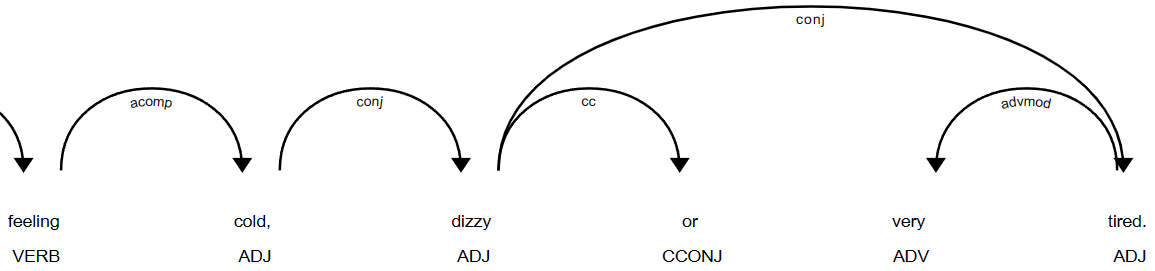
\includegraphics[width=\textwidth]{pictures/Dep_Parser.png}
    \caption{Dependency Parser}
    \label{fig:dep_parser}
\end{figure}

Es eröffnet sich damit eine einfache Methode, auch Symptome, die nicht im Trainingsvokabular enthalten sind, von \emph{spaCy} als Symptome erkennen zu lassen.

\subsubsection{Negationen}
\label{subsec: negations} 

In folgendem Satz wird fälschlich vom Medextractor erkannt, dass Interesse ein Symptom einer Depression ist:\\

\emph{\glqq The psychological symptoms of depression include having no motivation or interest in things.\grqq}\\

Dies liegt daran, dass der Medextractor nicht aus dem Zusammenhang erkennt, dass \emph{interest} in diesem Fall negiert ist, auch wenn das \emph{no} lediglich vor \emph{motivation}\ steht. 

\begin{figure}[h]
    \centering
    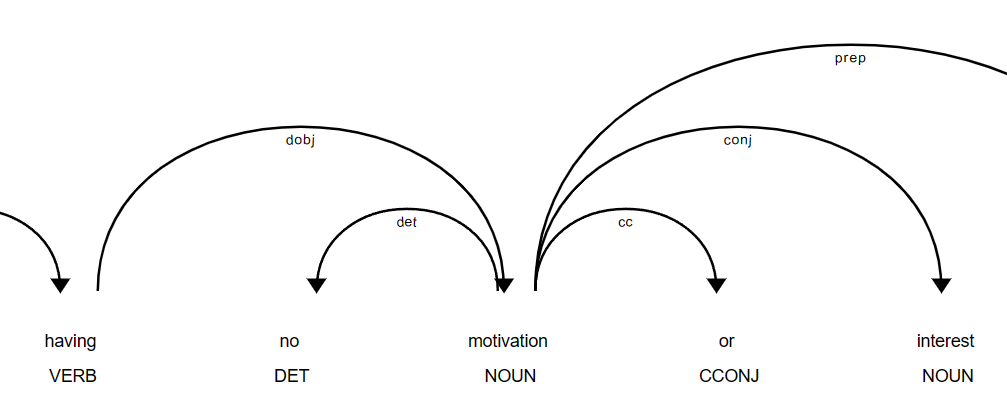
\includegraphics[width=\textwidth]{pictures/Dep_Parser_Negation.png}
    \caption{Dependency Parser bei Negation}
    \label{fig:negation}
\end{figure}

Abbildung \ref{fig:negation} zeigt, dass auch hier der Dependency Parser von \emph{spaCy} gute Dienste leisten kann. Er erkennt, dass \emph{motivation} und \emph{interest} über eine Konjunktion miteinander verbunden sind und dass \emph{no} damit sowohl die Begriffe {motivation} als auch \emph{interest} näher bestimmt.

\subsubsection{Korrelation zwischen Krankheit und Symptom}
\label{subsec: stigmatisierung} 

Kann von einer Krankheit relativ sicher auf Symptome geschlossen werden, so ist der umgekehrte Schluss von Symptom auf Krankheit häufig jedoch sehr unsicher. Ein Beispiel ist der Begriff \emph{anxiety} (Angst / Besorgnis). Bei der Analyse des Handbuchs findet der Medextractor diesen Begriff im Zusammenhang mit über 70 Krankheiten / Störungen. Dieser Umstand ermöglicht es einer Software, automatisch zu erkennen, dass ein Symptom oder Befund keinen sicheren Rückschluss auf eine Krankheit erlaubt. Auch kann durch Auswertung der Häufigkeit ein Modell entwickelt werden, um die Aussagekraft eines Befund zu bewerten.

Problematischer ist es aber z.B. mit dem Zusammenhang \emph{agoraphobia} - \emph{chest pain}, der in dem Satz:\\

\emph{\glqq The physical symptoms of agoraphobia can be similar to those of a panic attack and may include chest pain.\grqq}\\

gefunden wird. Da nur Texte über psychische Erkrankungen untersucht wurden, erscheinen Brustschmerzen nun als eindeutig der Agoraphobie (Angst vor großen Plätzen und Menschenansammlungen) zugeordnet zu sein. Würde man auch andere medizinische Texte untersuchen, so würde deutlicher werden, dass Brustschmerzen allein keinen deutlichen Hinweis auf eine Agoraphobie geben. Es erscheint daher sinnvoll, den Umfang analysierter Texte auf allgemeine medizinische Texte zu erweitern, auch wenn ein Projekt sich nur auf psychologische Themen beschränkt.

In vielen Fällen kann ein voreiliger Rückschluss von Symptom auf Krankheit auch zu Stigmatisierungen führen. So ist zwar ein dementer Mensch oft alt, alte Menschen dürfen aber nicht pauschal für dement gehalten werden. Da der Begriff \emph{aging} im Symptom-Vokabular enthalten ist, findet der Medextractor in dem Satz:\\

\emph{\glqq But dementia is not a normal part of aging.}\grqq\\

den Zusammenhang \emph{dementia} - \emph{aging}. Ähnlich verhält es sich mit dem Satz:\\

\emph{\glqq ...alcohol misuse can lead to social problems ... such as unemployment ...\grqq},\\

in dem der Zusammenhang \emph{alcohol misuse} - \emph{unemployment} gefunden wird. Auch wenn Alter und (Langzeit-)Arbeitslosigkeit keine unbegründeten Indikatoren für psychische Probleme sind, muss darauf geachtet werden, dass eine Software nicht stigmatisierend agiert. Hier kann wahrscheinlich nicht auf ein automatisches Erkennen gesetzt werden, sondern die Software-Entwickler müssen sicherstellen, dass ihre Software mit Begriffen wie Arbeitslosigkeit und Alter angemessen umgeht. Im Fall des Medextractors könnten solche Begriffe z.B. manuell aus dem Vokabular entfernt oder durch Einführung einen Attributes als problematisch markiert werden.

\subsubsection{Keine exakte Übereinstimmung zwischen Trainingsvokabular und Text}
\label{subsec: nomatch} 

In einigen Fällen werden Krankheiten und Symptome in einem Text nicht gefunden, obwohl ähnliche (aber nicht nicht genau gleiche) Begriffe im Trainingsvokabular enthalten sind. Gemäß Tabelle \ref{tab:vergleich_manuell_medextractor} wird z.B. der Zusammenhang \emph{\glqq ... changes to your menstrual cycle ....\grqq} und \emph{Depression} vom Medextractor nicht erkannt. Das Trainingsvokabular enthält jedoch mehrere relevante Einträge, etwa \emph{abnormal menstrual cycle} oder auch nur im Plural \emph{menstrual cycles}. Eine einfache, wenn auch nur in einigen Fällen wirksame Lösung, wäre es, den \emph{Lemmatizer} zu nutzen und sowohl Text als auch Trainingsvokabular in die Grundwörter zu überführen. In diesem Fall wäre dann auch der Begriff {menstrual cycle} im Singular im Trainingsvokabular enthalten und würde in dem Text über Depression gefunden, so dass zumindest der Zusammenhang \emph{depression} - \emph{menstrual cycle} erkannt würde.

\subsubsection{Bedeutung von Aussagen}
\label{subsec: bedeutung} 

Die einfache Auswertung der gefundenen Entitäten ermöglicht es dem Medextractor nicht, die Bedeutung von Sätzen richtig zu erfassen. In dem Artikel auf Wikipedia findet sich z.B. die Aussage:\\

\emph{\glqq These challenges came ... from gay rights activists who criticised the APA's listing of homosexuality as a mental disorder.\grqq}\\

Hier wird, da auch in dem \emph{MetaMapLite} Vokabular \emph{homosexuality} als Befund - aber nicht als Krankheit/Störung - enthalten ist, ein Zusammenhang zwischen Homosexualität und einer geistigen Störung gefunden. Dies entspricht aber natürlich nicht der Aussage des Satzes. Um die Bedeutung von Aussagen zu erfassen, ist ein höherer Aufwand zu treiben als in den bisherigen Beispielen. Ein Ansatz könnte sein, in den bisher gefundenen Beispielsätzen nach Satzmustern zu suchen, mit denen typischerweise Symptome beschrieben werden. Betrachten wir hierzu den Satz\\

\emph{\glqq Other typical symptoms of severe depression are changes in appetite.\grqq}\\

Hier wird \emph{changes in appetite} als Symptom und \emph{severe depression} als Krankheit gefunden. Dieser Satz beschriebe auch das Symptom einer Krankheit, wenn die Begriffe \emph{change of appetite} und \emph{severe depression} durch andere Begriffe aus dem Trainingsvokabular ersetzt würden. Allerdings sind auch viele Abwandlungen dieses Satzes denkbar und es sollte die Zielsetzung verfolgt werden, nach Möglichkeit nicht alle diese Abwandlungen trainieren zu müssen.

\begin{table}
\centering
\begin{tabular}{lllll}
\hline
\textbf{Text}	& \textbf{Lemma}	& \textbf{POS} & \textbf{TAG} & \textbf{DEP} \\
\hline
Other & other & ADJ & JJ & amod \\
typical & typical & ADJ & JJ & amod \\
symptoms & symptom & NOUN & NNS & nsubj \\
of & of & ADP & IN & prep \\
severe & severe & ADJ & JJ & amod \\
depression & depression & NOUN & NN & pobj \\
are & be & AUX & VBP & ROOT \\
changes & change & NOUN & NNS & attr \\
in & in & ADP & IN & prep \\
appetite & appetite & NOUN & NN & pobj \\
.  & . & PUNCT & . & punct \\
\hline
\end{tabular}
\caption{Ergebnis der \emph{spaCy}-Pipeline}
\label{tab:spaCy2}
\end{table}

Mit Hilfe der \emph{spaCy}-Pipeline können Sätze auf ihren Kerninhalt reduziert werden. Dazu wird ein Satz zunächst durch die Pipeline analysiert (s. Tabelle \ref{tab:spaCy2}). In obigem Beispiel wird als zentrales Verb (root) an Position 6 das Wort \emph{are} gefunden. \emph{spaCy} bietet Methoden, mit denen Eltern und Kinder von einzelnen Wörtern gefunden werden können. Die Kinder des Wortes \emph{are} sind z.B. \emph{symptoms} und \emph{changes} (Abbildung \ref{fig:typ_phrase}). 

\begin{figure}[h]
    \centering
    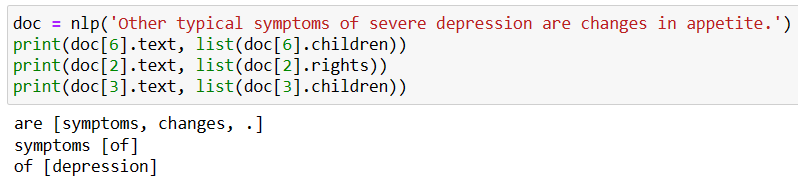
\includegraphics[width=\textwidth]{pictures/Dep_Parser_Text.png}
    \caption{Dependency Parser Ausgabe}
    \label{fig:typ_phrase}
\end{figure}

Man kann nun einen typischen Satz folgendermaßen charakterisieren:

\begin{enumerate}
	\item Die Wurzel (root) des Satzes muss entweder das Verb \emph{is} oder \emph{are} sein.
	\item Eines der Kinder der Wurzel muss als Lemma den Begriff \emph{symptom} besitzen.
	\item Das andere Kind\footnote{Es kann sich auch um mehrere Kinder (also Symptome) handeln.} muss ein Begriff aus dem Symptom-Vokabular sein (ggf. zusammengesetzt).
	\item Rechts neben dem Begriff mit Lemma \emph{Symptoms} steht das Wort \emph{of}.
	\item Das Kind des Begriffs \emph{of} muss ein Begriff aus dem Krankheiten-Vokabular sein (ggf. zusammengesetzt)
\end{enumerate}

Auf diese Weise können auch andere Satzkonstrukte festgelegt werden, mit denen üblicherweise die Symptome von Krankheiten beschrieben werden. Da der \emph{Dependency Parser} trainierbar ist, ist es möglich die hierarchische Gliederung von Sätzen auch anwendungsspezifisch erfolgen zu lassen, um dadurch das Auffinden typischer Sätze zu vereinfachen (vgl. Kapitel 10, Abschnitt `Creating a new Dependency Parser' in \cite{vasiliev2020natural}).

Nach all den Aufzählungen der Schwächen des Medextractors sei abschließend angemerkt, dass die sehr einfache Logik des Medextractors den Vorteil besitzt, dass alle Beziehungen von Krankheiten und Symptomen in einem Text gefunden werden, sofern die Begriffe im Vokabular enthalten sind. Die vom Medextractor gefundene Sammlung von Beispielsätzen ist daher eine gute Grundlage, um typische Sätze finden zu können.






\section{Zusammenfassung}
\label{sec:zusammenfassung_evaluierung} 

